\chapter{La crescita delle funzioni}

Il tasso di crescita del tempo di esecuzione di un algoritmo fornisce una semplice caratterizzazione dell'efficienza dell'algoritmo; inoltre, ci consente di confrontare le prestazioni relative di algoritmi alternativi.
Quanto operiamo con dimensioni dell'input abbastanza grandi da rendere rilevante soltanto il tasso di crescita del tempo di esecuzione, stiamo studiando l'efficienza \textbf{asintotica} degli algoritmi. In altre parole, ci interessa sapere come aumenta il tempo di esecuzione di un algoritmo al crescere della dimensione dell'input \textit{al limite}, quando la dimensione dell'input cresce senza limitazioni.

\section{Notazione asintotica}
Le notazioni che usiamo per descrivere il tempo di esecuzione  asintotico di un algoritmo sono definite in termini di funzioni il cui dominio è l'insieme dei numeri naturali $\mathbb{N}=\{0,1,2,3,\ldots\}$.

\subsection{Notazione Theta grande}

\dfn{Notazione Theta grande}{
	Per una data funzione $g(n)$, indichiamo con $\Theta(g(n))$ l'insieme delle funzioni:
	\begin{equation}\label{eq:theta_def}
		\Theta(g(n))= \biggl \{ f(n) \; | \; \exists c_{1},c_{2},n_{0} \in \mathbb{N} \Bigl( \forall n \geq n_{0} \bigl(0 \leq  c_{1}\cdot g(n) \leq f(n) \leq c_{2}\cdot g(n) \;\; \forall \; n \geq n_{0}\bigr) \Bigr) \biggl \}
	\end{equation}
}

Una funzione $f(n)$ appartiene all'insieme $\Theta(g(n))$ se esistono delle costanti positive $c_{1}$ e $c_{2}$ tali che possa essere ``racchiusa'' fra $c_{1}\cdot g(n)$ e $c_{2}\cdot g(n)$, per valori sufficientemente grandi di $n$. Poiché $\Theta (g(n))$ è un insieme, dovremmo scrivere ``$f(n) \in \Theta(g(n))$'' per indicare che la funzione $f(n)$ è un elemento di $\Theta(g(n))$. Invece, con un abuso di notazione, di solito si trova scritto ``$f(n)=\Theta(g(n))$'' per esprimere lo stesso concetto. Un altro modo per definire che $f(n)$ e $g(n)$ sono \textbf{asintoticamente equivalenti} è il seguente:
\begin{equation}\label{eq:theta2}
	f(n)=\Theta(g(n)) \iff \lim_{n \to +\infty} \frac{f(n)}{g(n)}=k > 0
\end{equation}

\begin{figure}[ht!]
	\centering
	\subfloat[\label{fig:notazioniasintotiche1}]{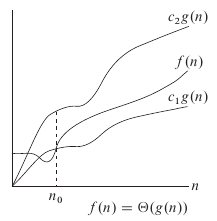
\includegraphics[scale=0.8]{res/Theta.jpg}} \quad
	\subfloat[\label{fig:notazioniasintotiche2}]{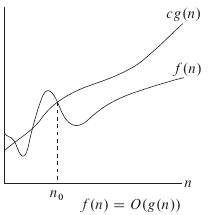
\includegraphics[scale=0.8]{res/Ogrande.jpg}} \quad
	\subfloat[\label{fig:notazioniasintotiche3}]{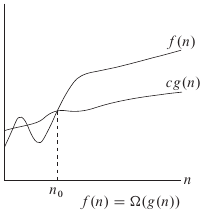
\includegraphics[scale=0.8]{res/Omega.jpg}}
	\caption{Esempi grafici delle notazioni $\Theta$, O grande e $\Omega$}
\end{figure}

La Figura \ref{fig:notazioniasintotiche1} presenta un grafico intuitivo delle funzioni $f(n)$ e $g(n)$, dove $f(n)=\Theta(g(n))$. Per tutti i valori di $n$ a destra di $n_{0}$, il valore di $f(n)$ coincide o sta sopra $c_{1}g(n)$ o sta sotto $c_{2}g(n)$. In altre parole, per ogni $n\geq n_{0}$, la funzione $f(n)$ è uguale a $g(n)$ a meno di un fattore costante. Si dice che $g(n)$ è un \textbf{limite asintoticamente stretto} per $f(n)$.


\begin{example}
		Dimostriamo che $\frac{1}{2}n^{2}-3n = \Theta(n^{2})$.
	Per farlo dobbiamo determinare le costanti positive $c_{1}$, $c_{2}$ e $n_{0}$ in modo che:
	\begin{displaymath}
		c_{1}n^{2} \leq \frac{1}{2}n^{2}-3n \leq c_{2}n^{2}
	\end{displaymath}

	per qualsiasi $n \geq n_{0}$. Dividendo per $n^{2}$, si ha:
	\begin{displaymath}
		c_{1} \leq \frac{1}{2}-\frac{3}{n} \leq c_{2}
	\end{displaymath}

	La disuguaglianza destra può essere resa valida per qualsiasi valore di $n \geq 1$ scegliendo una costante $c_{2}\geq \frac{1}{2}$.

	Analogamente, la disuguaglianza sinistra può essere resa valida per qualsiasi valore di $n \geq 7$ scegliendo una costante $c_{1} \leq \frac{1}{14}$. Quindi scegliendo $c_{1}=\frac{1}{14}$, $c_{2}=\frac{1}{2}$ e $n_{0}=7$, possiamo verificare che $\frac{1}{2}n^{2}-3n = \Theta(n^{2})$.

\end{example}

\subsection{Notazione O grande}
La notazione $\Theta$ limita asintoticamente una funzione da sopra e da sotto. Quando invece abbiamo soltanto un \textbf{limite asintotico superiore}, utilizziamo la notazione O grande.

\dfn{Notazione O grande}{
	Per una data funzione $g(n)$, denotiamo con $O(g(n))$ l'insieme delle funzioni:
	\begin{equation}
		O(g(n))= \biggl \{ f(n)\; | \; \exists  c, n_{0} \in \mathbb{N}  \Bigl( \forall \; n \geq n_{0} \bigl(0 \leq f(n) \leq cg(n) \bigr)  \Bigr) \biggl \}
	\end{equation}
}
La notazione O si usa per assegnare un limite superiore a una funzione, a meno di un fattore costante. Un altro modo per definire che $f(n)$ \textit{non cresce più velocemente} di $g(n)$ è il seguente:
\begin{equation}
	f(n)=O(g(n)) \iff \lim_{n \to +\infty} \frac{f(n)}{g(n)}=0
\end{equation}
La funzione $g(n)$ è quindi un infinito superiore rispetto a $g(n)$. La figura \ref{fig:notazioniasintotiche2} illustra il concetto intuitivo che sta dietro questa notazione. Per qualsiasi valore n a destra di $n_{0}$, il valore della funzione $f(n)$ coincide o sta sotto $cg(n)$.

\begin{osservation}
	Notiamo che $f(n)=\Theta(g(n)) \implies f(n)=O(g(n))$, in quanto la notazione $\Theta$ è una notazione più forte della notazione O. Secondo la notazione degli insiemi possiamo scrivere $\Theta(g(n)) \subseteq O(g(n))$.
\end{osservation}

\subsection{Notazione Omega grande}
Così come la notazione O grande fornisce un limite asintotico \textit{superiore} a una funzione, la notazione $\Omega$ fornisce un \textbf{limite asintotico inferiore}.

\dfn{Notazione Omega grande}{
	Per una data funzione $g(n)$, denotiamo con $\Omega(g(n))$ l'insieme delle funzioni
	\begin{equation}
		\Omega(g(n))= \biggl \{ f(n)\; | \; \exists c,n_{0} \in \mathbb{N} \Bigl( \forall \; n \geq n_{0} \bigl( 0 \leq cg(n) \leq f(n) \;\; \bigr) \Bigr)  \biggr \}
	\end{equation}
}

Un altro modo per dire che $f(n)$ \textit{non cresce più lentamente} di $g(n)$ è attraverso il seguente limite che esprime il fatto che $g(n)$ è un infinito superiore rispetto a $f(n)$:
\begin{equation}
	f(n)=\Omega(g(n)) \iff \lim_{n \to +\infty} \frac{f(n)}{g(n)}= + \infty
\end{equation}

Il concetto intuitivo che sta dietro la notazione $\Omega$ è illustrato nella figura \ref{fig:notazioniasintotiche3}. Per tutti i valori di n a destra di $n_{0}$, il valore di $f(n)$ coincide o sta sopra $cg(n)$.

\subsection{Proprietà delle relazioni asintotiche}
Molte delle proprietà delle relazioni fra numeri reali si applicano anche ai confronti asintotici. Supponiamo che $f(n)$ e $g(n)$ siano asintoticamente positive.

\begin{teorbox}[Proprietà transitiva]
		Valgono le seguenti proprietà:
	\begin{eqnarray}
		f(n)=\Theta(g(n)) \wedge g(n)=\Theta(h(n)) \implies f(n)=\Theta(h(n)) \\
		f(n)=O(g(n)) \wedge g(n)=O(h(n)) \implies f(n)=O(h(n)) \label{eq:O_transitivity}\\
		f(n)=\Omega(g(n)) \wedge g(n)=\Omega(h(n)) \implies f(n)=\Omega(h(n))
	\end{eqnarray}
\end{teorbox}
\begin{proof}
	Dimostriamo per comodità la \ref{eq:O_transitivity}, le altre proprietà si dimostrano in modo analogo. Per definizione di O grande:
	\begin{eqnarray}
		\exists n_{0} > 0 \quad \exists c_{1}>0 \quad \forall n \geq n_{0} \quad f(n)\leq c_{1}g(n) \nonumber \\
		\exists n_{1} > 0 \quad \exists c_{2}>0 \quad \forall n \geq n_{0} \quad g(n)\leq c_{2}h(n) \nonumber
	\end{eqnarray}
	Assumendo queste due formule vere fissiamo $n_{2}=\mbox{max}\{n_{0},n_{1}\}$ quindi
	\begin{displaymath}
		\exists n_{2} > 0 \quad \exists c_{1},c_{2}>0 \quad \forall n \geq n_{2} \quad f(n)\leq cg(n) \quad \wedge \quad g(n) \leq c_{2}h(n)
	\end{displaymath}
	Maggiorando:
	\begin{displaymath}
	f(n) \leq c_{1}c_{2}h(n)
	\end{displaymath}
	Ponendo $\overline{c}=c_{1}c_{2}$ si ottiene
	\begin{displaymath}
		\exists n_{2} > 0 \quad \exists \overline{c}>0 \quad \forall n \geq n_{2} \quad f(n) \leq \overline{c}h(n)
	\end{displaymath}
	Quindi $f(n)=O(h(n))$.
\end{proof}


\begin{teorbox}[Proprietà riflessiva]
		Valgono le seguenti proprietà:
	\begin{eqnarray}
		f(n)=\Theta(f(n)) \\
		f(n)=O(f(n)) \\
		f(n)=\Omega(f(n))
	\end{eqnarray}
\end{teorbox}

\begin{teorbox}[Proprietà simmetrica]
		Vale la seguente proprietà
	\begin{equation}
		f(n)=\Theta(g(n)) \Leftrightarrow g(n)=\Theta(f(n))
	\end{equation}
\end{teorbox}


	Dalla definizione di notazione $\Theta$:
	\begin{equation}
		\exists n_{0}>0 \quad \exists c_{1},c_{2} > 0 \quad c_{1}g(n) \leq f(n) \leq c_{2}g(n)
	\end{equation}
	possiamo estrarre delle costanti utili per dimostrare il teorema, infatti:
	\begin{eqnarray}
		c_{1}g(n) \leq f(n) \leftrightarrow f(n) \leq \frac{1}{c_{1}} f(n) \nonumber \\
		f(n) \leq c_{2}g(n) \leftrightarrow \frac{1}{c_{2}} \leq g(n) \nonumber \\
	\end{eqnarray}
	quindi ponendo
	\begin{eqnarray}
		c_{3}=\frac{1}{c_{1}} \nonumber \\
		c_{4}=\frac{1}{c_{2}} \nonumber
	\end{eqnarray}
	possiamo scrivere
	\begin{equation}
		\exists n_{0}>0 \quad \exists c_{3},c_{4} > 0 \quad c_{4}f(n) \leq g(n) \leq c_{3}f(n)
	\end{equation}
	ovvero $g(n)=\Theta(f(n))$.
\begin{flushright}
	\blacksquare
\end{flushright}

\begin{teorbox}[Simmetria trasposta]
		Vale la seguente proprietà
	\begin{equation}
		f(n)=O(g(n)) \Leftrightarrow g(n)=\Omega(f(n))
	\end{equation}
\end{teorbox}

\section{Ricerca delle costanti mediante metodo grafico}
Attraverso la definizione mediante limite delle notazioni O grande, $\Theta$ e $\Omega$ è possibile ottenere un metodo per la ricerca delle costanti $c_{1}$, $c_{2}$ ed $n_{0}$ senza dover applicare necessariamente la definizione analitica. Infatti, posto $$h(n)=\frac{f(n)}{g(n)}$$ è possibile studiare il grafico della sua funzione per ottenere le costanti ricercate.
Osserviamo infatti che, se $f(n)=\Theta(g(n))$ allora vale
\[
\exists n_{0} \quad \exists c_{1},c_{2}>0 \quad \forall n>n_{0} \quad c_{1}g(n)<f(n)<c_{2}g(n)
\]
dividendo per $g(n)$ si ottiene:
\[
\exists n_{0} \quad \exists c_{1},c_{2}>0 \quad \forall n>n_{0} \quad c_{1}<\frac{f(n)}{g(n)}<c_{2}
\]
e sostituendo il rapporto $\frac{f(n)}{g(n)}=h(n)$ :
\[
\exists n_{0} \quad \exists c_{1},c_{2}>0 \quad \forall n>n_{0} \quad c_{1}<h(n)<c_{2}
\]
Il metodo grafico consiste nella ricerca delle due costanti $c_{1}$ e $c_{2}$ che delimitano l'andamento asintotico della funzione $h(n)$. Supposto quindi che esista e sia limitato il limite
\[
\lim_{n \to +\infty} h(n)= \; l >0
\]
si ottiene che la retta $y=l$ è un asintoto orizzontale per la funzione $h(n)$.

Per tale asintoto possono presentarsi tre situazioni:
\begin{enumerate}
	\item \textbf{$h(n)$ tende a $y=l$ dall'alto.} Scelto un $n_{0}$ in cui la funzione $h(n)$ è \textit{decrescente in un intervallo illimitato} si prendono i valori
	\[
	\begin{cases}
		y=h(n_{0}) \\
		l
	\end{cases}
	\]
	che individuano le due costanti che fanno valere la disuguaglianza $$c_{1}\leq h(n) \leq c_{2}$$
	\item \textbf{$h(n)$ tende a $y=l$ dal basso.} Si procede in maniera analoga al caso precedente, però oltre allo studio della monotonia mediante la derivata prima sarà necessario studiare anche il \textbf{segno della funzione} dato che siamo alla ricerca di \textit{costanti positive}. All'interno della semiretta a destra dove la funzione assume segno positivo si può scegliere a piacere un punto $x_{t}$ e valutare la funzione in quel punto: $y_{1}=h(x_{t})$. Quindi l'insieme delle costanti $(y_{1},l)$ rappresenta una coppia di costanti che garantiscono la proprietà da dimostrare.
	\item \textbf{$h(n)$ tende a $y=l$ in modo oscillante.} In questo caso, poco frequente, $n_{0}$ si deve trovare nell'intervallo in cui l'oscillazione si smorza. All'interno di questo intervallo andiamo a selezionare i valori di minimo e massimo locale.
	
\end{enumerate}
	\begin{figure}[ht!]
		\centering
	\subfloat[Caso 1: $h(n)$ tende al limite dall'alto]{\includegraphics[scale=0.8]{res/asintoto_orizzontale2}}\qquad
	\subfloat[Caso 2: $h(n)$ tende al limite dal basso]{\includegraphics[scale=0.8]{res/asintoto_orizzontale1}}\qquad
	\subfloat[Caso 3: $h(n)$ tende al limite in modo oscillante]{\includegraphics[scale=.8]{res/asintoto_orizzontale3}}
	\caption{}
\end{figure}

\begin{example}
	Siano
	\[
	\begin{array}{l}
		f(n)=n \\
		g(n)=4n-10
	\end{array}
	\]
	Dimostriamo attraverso il metodo grafico che vale $$g(n)=\Theta(f(n))$$

	Si calcola innanzitutto il limite
	\begin{equation}\label{limit1}
		\lim_{n \to \infty} \frac{4n-10}{n}= 4
	\end{equation}


	Esiste quindi un asintoto orizzontale di equazione $y=4$. Siamo interessati alla ricerca delle due costanti che verificano la condizione:
	\begin{equation}\label{disuguaglianza1}
		\exists n_{0} >0 \quad \exists c_{1},c_{2}>0 \quad c_{1}n \leq 4n-10 \leq c_{2}n \quad \forall n > n_{0}
	\end{equation}

	Studiamo quindi la monotonia della funzione $h(n)=\frac{4n-10}{n}$:
	$$
	h'(n)= \frac{10}{n^{2}} > 0 \quad \forall n>0
	$$
	La funzione quindi è strettamente crescente in tutto l'intervallo $(0,+\infty)$
	Per cercare due costanti positive è necessario che la funzione $h(n)$ sia positiva
	$$
	h(n)=\frac{4n-10}{n}>0 \quad \iff \quad n> \frac{5}{2}
	$$
	Prendendo a piacere un $n_{0}$ all'interno dell'intervallo $(\frac{5}{2}, +\infty)$ si troveranno quindi due costanti $c_{1}$ e $c_{2}$ che verificano la disuguaglianza \ref{disuguaglianza1}. Infatti, preso $n_{0}=3$ si valuta la funzione $h(n)$ in quel punto ottenendo $$h(3)=\frac{4\cdot3-10}{3}=\frac{2}{3}$$ mentre la costante $c_{2}$ era stata data dal limite \ref{limit1}.
\end{example}